
\documentclass[12pt]{article}
\usepackage[left=25mm, top=20mm, right=10mm, bottom=30mm]{geometry}
\usepackage[utf8]{inputenc}
\usepackage{authblk}
\usepackage{mathtools}
\usepackage{forloop}
\usepackage{pgfplots}
\usepgfplotslibrary{colormaps}
\pgfplotsset{width=16cm,compat=newest,}
\title{	\raggedright\Large\textbf{Exploring Quantum Systems for Pseudo-Random\\
	Number Generation}}
\author[1,a]{\raggedright\small\textbf{Luis Jose Mantilla Santa Cruz}}
\author[1,b]{\textbf{Luis F. Faina}}
\author[1,c]{\textbf{ Joao Henrique de Souza Pereira}}
\affil[1]{Federal University of Uberlandia, Faculty of Computing, Uberl andia, Minas Gerais, Brazil}
\affil[a]{\textit{luis.santa@ufu.br}}
\affil[b]{\textit{luisfaina@ufu.br}}
\affil[c]{\textit{joaohs@ufu.br}}
\date{}
\begin{document}
	\maketitle
	{\raggedright\large\textbf{Abstract}}\\
	
	{Quantum realizations have opened a new ways for computer science. The new characteristics and phenomenons allow us to
	create new algorithms for general proposes. An interesting topic is random number generation. There are two perspectives for
	this proposes. True random numbers generator (TRN) and pseudo random numbers generator (PRNG). True Random Number
	Generators has four significant characteristics: randomness, long Period, insensitivity to seeds, repeatability. Additionally,
	Pseudo Random Number Generators is a fascinating topic that leverages the principles of computer science to craft deterministic
	algorithms, enabling the creation of a sequence of pseudo-random numbers. A crucial element in this process is the ’seed’,
	which serves as the initial value to generate the entire sequence. This document proposes a algorithm based on a quantum
	system and the quasi-probability of its possible states to generate a long set of numbers which has pseudo random properties.
	The quantum system is compound by n qubits, its initial conditions and a small set of rotation gates with a fixed angle. The
	tests were realized using the battery test called NIST SP800-22, and $\alpha$ = 0.01 as a threshold to ensures 99% of precision. The
	results demonstrate that it is possible generate a long set of pseudo numbers with random characteristics using a quantum
	simple operation. However, the experiments reveal that a real world implementation require a quantum system with at least
	10-9 precision order.}\\
	
	{\raggedright\large\textbf{Introduction}}\\
	
	{Quantum technology offers several new features and has opened the door to a new era - the quantum age. This age began in the early 1980s, when Benioff and Feynman introduced the concept of quantum computing, the main consequencce of the use of quantum mechanism for this propose is the creation of a more effective computer. This theoretical machine is based on qubits as the minimum information unit. Additionally, it has the ability of work with an exponential number of states and realize bast calculations in short time. This new characteristics and phenomenons makes possible the quantum supremacy.\par
	A quantum system is compound by a set of qubits, its initial parameters and the gates destinated to realize changes the qubits. The first component is the qubit which has the property of being in a linear combination of its single states, it means $\mid \psi⟩ = \alpha \mid 0⟩+\beta \mid$ 1⟩, where it’s complex components have the restriction $\parallel \alpha \parallel^2 +\parallel \beta \parallel^2 = 1$. An additional consequence is that
	each auditioned qubit increment exponentially the number of possible states of the system. The second component is the unitary
	operator which is compound of quantum gates. It allows us to explore the Hilbert’s space by making changes into the qubits.
	The third component is the measurement that makes the system collapse. However, quantum computing requires a change of
	paradigm for including new quantum phenomenons as part of regular algorithms to develop the counter part of traditional ones.\par
	As consequence of the realization of quantum computers, some new computer science areas were created: quantum
	communications, quantum computing, quantum sensing, and quantum simulation.\par
	Quantum computing aims to create a counterpart of traditional computing and incorporate new properties such as superposition, entanglement, squeezing, and coherence into algorithms. Some important subareas include quantum circuits and software,
	quantum hardware, quantum machine learning, and quantum information science. Some of these new methods, techniques, and
	algorithms are being used to solve real-world optimization problems4–6.\par
	Quantum communication focuses on the development of a new generation of functional communication networks and
	quantum information study the capacity of the quantum systems to express information, its associated mechanism, and its
	security. To achieve this goal, researchers deal with quantum entanglement, quantum teleportation, necessary quantum hardware,
	methods to improve network efficiency, quantum information, quantum cryptography, post quantum cryptography and other
	related issues.\par
	Random numbers has importance for our lives because many of the real world applications which are used every day
	requires of it. The definition of generated numbers has four important properties i) Randomness, ii) Long-period, iii) Insensitive 1
	to seeds, iv) Repeatability. In addition, many relevant events which have had an impact in economy, human right and others
	have occurred because the random systems were broken7.\par
	There exists two categories to generate random numbers. First, True-Random Number Generator (TRNG) which uses
	physical sources of true randomness to generate random numbers. Second, Pseudo-Random Number Generator (PRNG) which
	uses a deterministic algorithm to generate a set of numbers.\par
	TRNGs operate on the principle that certain physical phenomena, such as electronic noise, radioactive decay, or chaotic
	systems, are fundamentally unpredictable. These devices capture and convert these naturally occurring processes into random
	numbers. As a result, TRNGs provide numbers that are statistically independent and uniformly distributed, making them
	suitable for applications requiring the highest level of randomness and security.\par
	The key advantage of TRNGs is their resistance to predictability, ensuring that the generated numbers cannot be determined,
	even with complete knowledge of the generator’s internal state. This characteristic makes TRNGs invaluable in fields such as
	cryptography, secure communications, and gambling, where true randomness is essential to prevent exploitation or predictability.
	However, TRNGs may have limitations in terms of speed and efficiency due to their reliance on physical processes. Despite
	these limitations, they remain the preferred choice for applications where uncompromising randomness is paramount.\par
	Conversely, a Pseudo Random Number Generators (PRNGs) are a class of algorithms used to generate sequences of
	numbers that appear random but are, in fact, generated deterministically. These generators rely on initial values, called seeds,
	and a series of mathematical operations to produce a sequence of numbers that exhibit statistical properties resembling those of
	truly random sequences. While PRNGs can appear random, they are fundamentally driven by algorithms and initial seed values,
	meaning that their entropy evolves according to a predictable path.\par
	PRNGs are widely employed in various applications, including simulations, computer graphics, and statistical modeling.
	They offer several advantages, such as speed and repeatability, as the same seed will always produce the same sequence. This
	predictability can be beneficial in applications where reproducibility is desired.\par
	Some traditional algorithms were proposed: Yarrow 160, Fortuna, Blum Blum Shub, Counter-Based8. Some new algorithms
	for criptography based on quantum algorithms was proposed. The most common algorithm modify for this propose is quantum
	walks9–14. Additionally, new devices based on quantum technology such as QRNG JUR017 was presented and commercialized.\par
	The main limitation of PRNGs lies in their deterministic nature. Given the same initial seed, a PRNG will always produce
	the same sequence, which makes them unsuitable for applications requiring true randomness and security against predictability.
	Moreover, PRNGs can exhibit periodicity, where the sequence repeats after a certain number of values.\par
	This document is structured into several key sections. It begins with an introductory exploration of quantum computing.
	Subsequently, the Results section provides a summary of the theoretical analysis of the probabilities generated by a quantum
	system, along with the associated statistical tests. The subsequent section is dedicated to the discussion, where the obtained
	results are analyzed in comparison with JUR01, including discussions on advantages, disadvantages, and the analysis of the
	nature of the a non-uniform probability distribution by $\triangle H '(A)$. The following section is the conclusion, summarizing the main
	points. Finally, the document introduces and details the Quantum Quasi-Probability Pseudo Random Generator (QQ-PRG) algorithm for generating pseudo-random numbers.}\\
	
	{\raggedright\large\textbf{Results}}\\\\
	{\raggedright\small\textbf{Generation of long set of numbers pseudo random numbers}}\par
	{The method for generating an extensive list of numbers is analogous to other methods. It is grounded in the resultant
		quasi-probabilities of the states in a quantum system and a loop which makes possible to obtain a long list of numbers.\par
		To generate a sequence of numbers with random characteristics, a quantum system is initialized, and a sequence of quantum
		gates is applied sequentially to manipulate the quasi-probabilities of the quantum states. To obtain the pseudo random number,
		the first $n \geq 6$ most significant elements of the resulting probabilities for each state are discarded, and the next $k > 3$ precision
		elements are selected as the random number. Each generated number is then appended to the list of numbers.\par
		This method presents an strong dependence on the initial configuration of the quantum system, the initial parameters ’seed’,
		and the set of sequential gates. It dependence also compromise the security of the method due it is necessary know this three
		parameters to get all the numbers sequence.\par
		This method uses a quantum system to obtain its quasi-probability, its main advantage is given by the number of possible
		quantum states. The first restriction for the method is related to the quasi probability precision due it must be at least $10^{-9}$. The second restriction is given by the number of possible states and it’s quasi-probability due as more qubits are included into the
		system more divided is the information into the states. This phenomenon makes possible the occurrence of states with close to
		0 probability.}\\\\
		{\raggedright\small\textbf{Probability distribution analysis}}\par
		{In this subsection presents an analysis of two possibilities for probability distribution. First a uniform probability distribution
			which describe a true random number generator. Second a non-uniform probability distribution which describe the probability
			into a pseudo random number generator.}\\\\
	   	{\raggedright\small\textbf{Uniform Quantum Probability Distribution with Hadamard Gate}}\par
	   	{In this context, the quantum probability distribution is divided uniformly into 2
	   		n quantum states, ensuring that $\sum_{i=1}^{2^n} P(a_i)=1$.
	   		This equal division of probability can be likened to complete uncertainty within the quantum system, where each possibility
	   		holds equal likelihood, akin to a pure random system.\par
	   		Quantum computers achieve this uniform distribution by utilizing a fundamental quantum gate known as the Hadamard
	   		gate. The Hadamard gate demonstrates its ability to generate a 50\% chance of measuring the quantum state $\mid$0⟩ and an equally
	   		50\% chance of measuring $\mid$1⟩. This property serves as the foundation for the proposal put forth in a study by Kumar et al.15.
	   		The document establishes that leveraging multiple Hadamard gates can lead to the creation of random sequences of numbers.\par
	   		This approach illustrates the potential for a True Random Number Generator (TRNG) to be realized using a quantum
	   		computer. By harnessing the inherent unpredictability of quantum systems, this method paves the way for applications
	   		demanding the highest level of randomness and security, such as in cryptography and secure communications.\par
	   		Additionally, Shannon’s entropy serves as a metric to quantify the uncertainty or randomness inherent in a probability
	   		distribution16. In the context of a uniform quantum probability distribution, entropy is defined as \small$$H(A)=H(P(a_1),P(a_2)),...,P(a_{2^n}))=-\sum_{i} P(a_i)\log_2 P(a_i)\eqno(1)$$\par  In the case of a truly random process, the probability values are identical for every element, indicating maximal uncertainty.
	   		Therefore, for a quantum system, we have $H(A) \equiv H(P(a_1)) = H(P(a_2)) = ... = H(P(a_{2^n}
	   		))$.\par
	   		A uniform distribution within a quantum system, consisting of 2n
	   		elements observed over N shots, can be represented as$$ H(A)=\sum_{i=1}^{2^n} H(\frac{1}{2^n})\eqno(2)$$where $P(a_i)=\frac{1}{2^n}, i=1,...,2^n$
	   		. This representation is utilized throughout the document, with some modifications and
	   		constraints to effectively depict non-uniform probability distributions.\par
	   		Table 1 provides estimates for a uniformly distributed probability process within a quantum system. Notably, this perspective
	   		emphasizes that the introduction of extra qubits into the system leads to a partitioning of the total probability among an expanding
	   		set of states. It is essential to recognize that the uniform distribution not only divides the probability but also signifies that the
	   		system achieves maximum entropy. This maximum entropy is equivalent to the number of potential states within a quantum
	   		system, as demonstrated in Equation 6.}
	 		\begin{center}
	 			\begin{tabular}{ |c|c|c|c| } 
	 				\hline
	 				Qubits  & Possible States  & Probability & Shannon’s Entropy\\
	 				\hline
	 				1 & 2 & 0.5000 & 1 \\ 
	 				2 & 4 & 0.5000 & 2 \\ 
	 				3 & 8 & 0.3750 & 3 \\ 
	 				4 & 16 & 0.2500 & 4 \\ 
	 				5 & 32 & 0.1563 & 5 \\ 
	 				\hline
	 			\end{tabular}
	 		\end{center}
	   		{Table 1. Estimates for qubit numbers, possible states, mean probability, and corresponding Shannon’s entropy in a random
	   		system.\\\par
	   		Furthermore, Figure 1 provides a visual representation of the previously computed data. This visualization illustrates the
	   		two primary approaches to random number generation. The blue line depicts the entropy for a true random generator based on a
	   		specific number of qubits. In contrast, the red area represents the potential entropy achievable by a pseudo-random number
	   		generator within a quantum system. This straightforward visualization serves as compelling evidence of the extensive array of
	   		possibilities for developing PRNGs based on quantum technology.}\\
	   		
	   		
	   		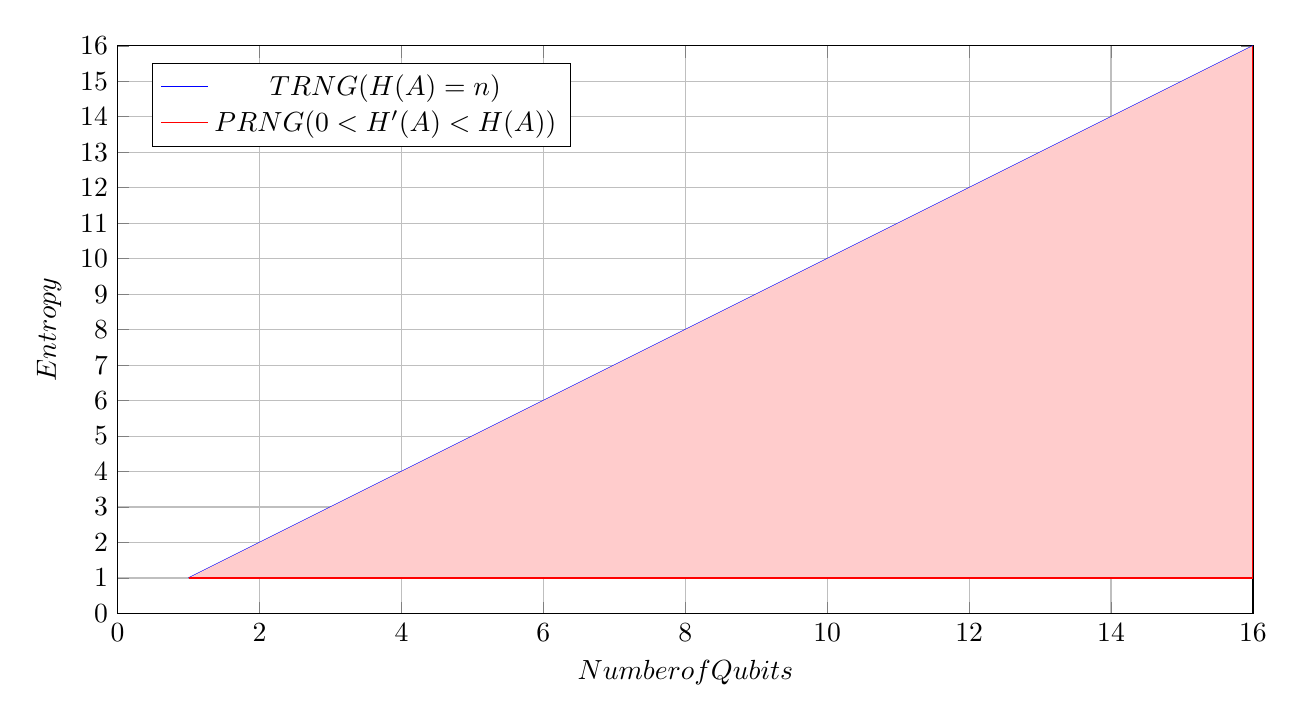
\begin{tikzpicture}
	   		
	   			\begin{axis}[
	   				xtick distance=2,
	   				ytick distance=1,
	   				legend pos = north west, 
	   				xlabel = {$Number of Qubits$},
	   				ylabel = {$Entropy$},
	   				ymax=16,
	   				ymin=0,
	   				xmax=16,
	   				xmin=0,
	   				grid=major,
	   				unit vector ratio = 2 1
	   				]
	   			\legend{ 
	   				$TRNG (H(A)=n)$ ,
	   				$PRNG(0<H'(A)<H(A))$, 
	   			};
	   				\addplot[blue] coordinates {
	   					(1,1)  (16,16)
	   				};
	   				\addplot[red] coordinates {
	   					(1,1)(1,1)  (16,1)(16,16)
	   				};
	   				\addplot[const plot,fill=red!20] coordinates {
	   					(1,1)  (16,16)
	   				};
	   				\addplot[red] coordinates {
	   					(1,1)(1,1)  (16,1)(16,16)
	   				};
	   			\end{axis}
	   		\end{tikzpicture}\\
	   	 	{Figure 1. This figure illustrates the entropy of True Random Number Generators (TRNGs) and Pseudo Random Number
	   	 		Generators (PRNGs) in a quantum system with varying numbers of qubits. The blue curve represents TRNGs with H(A) = n,
	   	 		while the red area corresponds to PRNGs with $0 < H'(A) < H(A)$.}
	   	 	
	   		
	   	
   		
	   		
	   		
	
\end{document}
